\documentclass{article}

\usepackage{graphicx}
\usepackage{booktabs}
\author{Jan Ruman}
\date{10.7.2021}
\title{Analysis of activations in neural networks}

\begin{document}

\maketitle
\author
\date

\begin{abstract}
    In this work, we attempt to analyze the properties of activations inside
    a neural network. 
\end{abstract}

\section{Introduction}
A neural network applies a sequence of non-linear transformations to its
input in order to produce an output. This procedure can be (and is)
done for all examples in the dataset. By storing the intermediate
transformations, we end up with multiple different representations of the
original dataset (possibly compressed and/or missing some information).

This work aims to analyze these representations in terms of their structure.
We are primarily interested in the way examples with the same class are
distributed when using the new representations.

\section{Methodology}
We will compare the data representations across two dimensions:
1) the depth of layer from which the representations were acquired and
2) whether the network was or was not trained. This means we will need
a neural network to be trained and datasets to train it on.

The representations are going to have many dimensions - it will be more
practical to use dimensionality reduction techniques that retain the
structure of the data. For that purpose, we are going to use t-SNE and UMAP
algorithms.

We need some way of comparing the structure of different representations.
Plotting embeddings acquired using dimensionality reduction techniques is
one of them, but some more rigorous approaches will be necessary to acquire
more reliable results. In order to measure the quality of a representation,
i.e., how well it clusters the same examples together and keeps different
examples away, we introduce several metrics in the next section.

A simple feedforward neural network with ReLU activations and three hidden
layers will be used. The widths of these layers are as follows: 512, 256, and
128 neurons.

We are going to use MNIST and FashionMNIST datasets.

\section{Embedding quality}
To measure the quality of a representation, we introduce several metrics that
capture the representation's properties. These properties then indicate how
good the representation is.

All except the last metric have distance as a unit. This is potentially
problematic as the absolute distance between points tells us nothing if we
do not know the distances between other points. It is thus necessary
to divide each of these metrics by the average distance between two points;
this will ensure that even though two embeddings have different scales, we
can still compare their metrics.

\subsection{Distances between points}
The first two metrics are concerned with an average distance between two points.
An average distance between points of the same class (\(d_s\)) and an average
distance between points of different classes (\(d_d\)) are measured. It is
quite obvious which one we would like to minimize and which one to maximize.

\subsection{Cluster centroids}
We can look at points belonging to the same class as a cluster. We introduce
two metrics using centroids of these clusters: 1) the total distance from 
points of a class to its centroid (\(c_s\)) and 2) the total distance between
different centroids (\(c_d\)).

\subsection{k-nearest neighbors}
We can use the k-nearest neighbors algorithm on the embedding to classify
examples in the dataset. The accuracy of k-nn (\(acc_{knn}\)) should
correlate with the quality of the embedding.

\section{Results}
Results presented in this part were acquired by running the
\texttt{\\ scripts/activations\_feedforward.py} script. Output of this script
used in this document is part of the repository; rerunning the script might
give slightly different results.

It is important to note that layer 0 refers to the input of the network.

\subsection{MNIST}
First, we will look at embeddings produced by t-SNE - these correspond
to Figure 1 and Figure 2. 

\begin{figure}
  \centering
    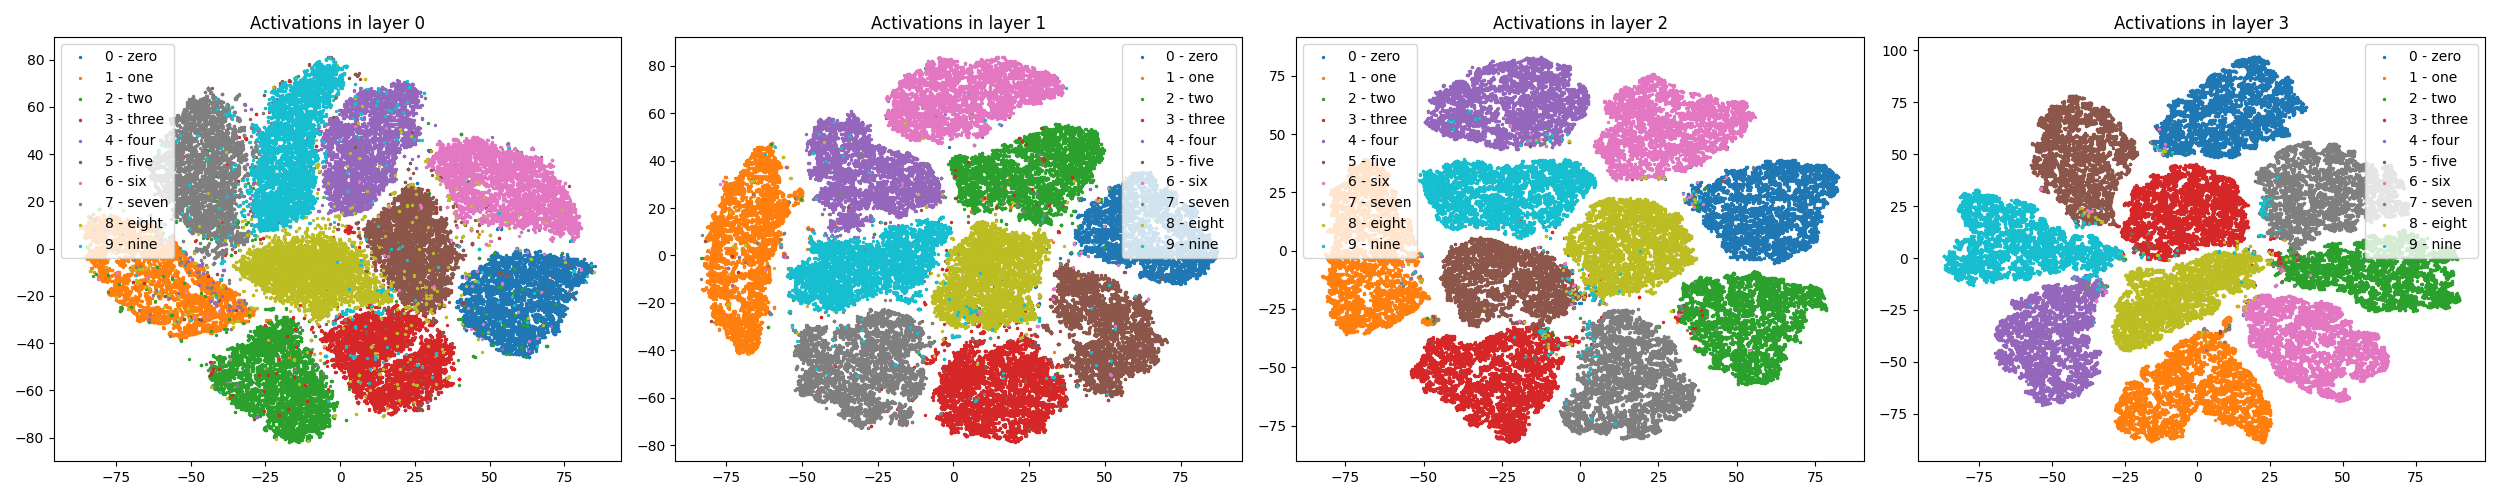
\includegraphics[width=1.0\textwidth]{../../out/activations_feedforward/mnist_t-sne_trained.png}
    \caption{Embeddings of activations in layers of a neural network trained on MNIST (t-SNE).}
\end{figure}

\begin{figure}
  \centering
    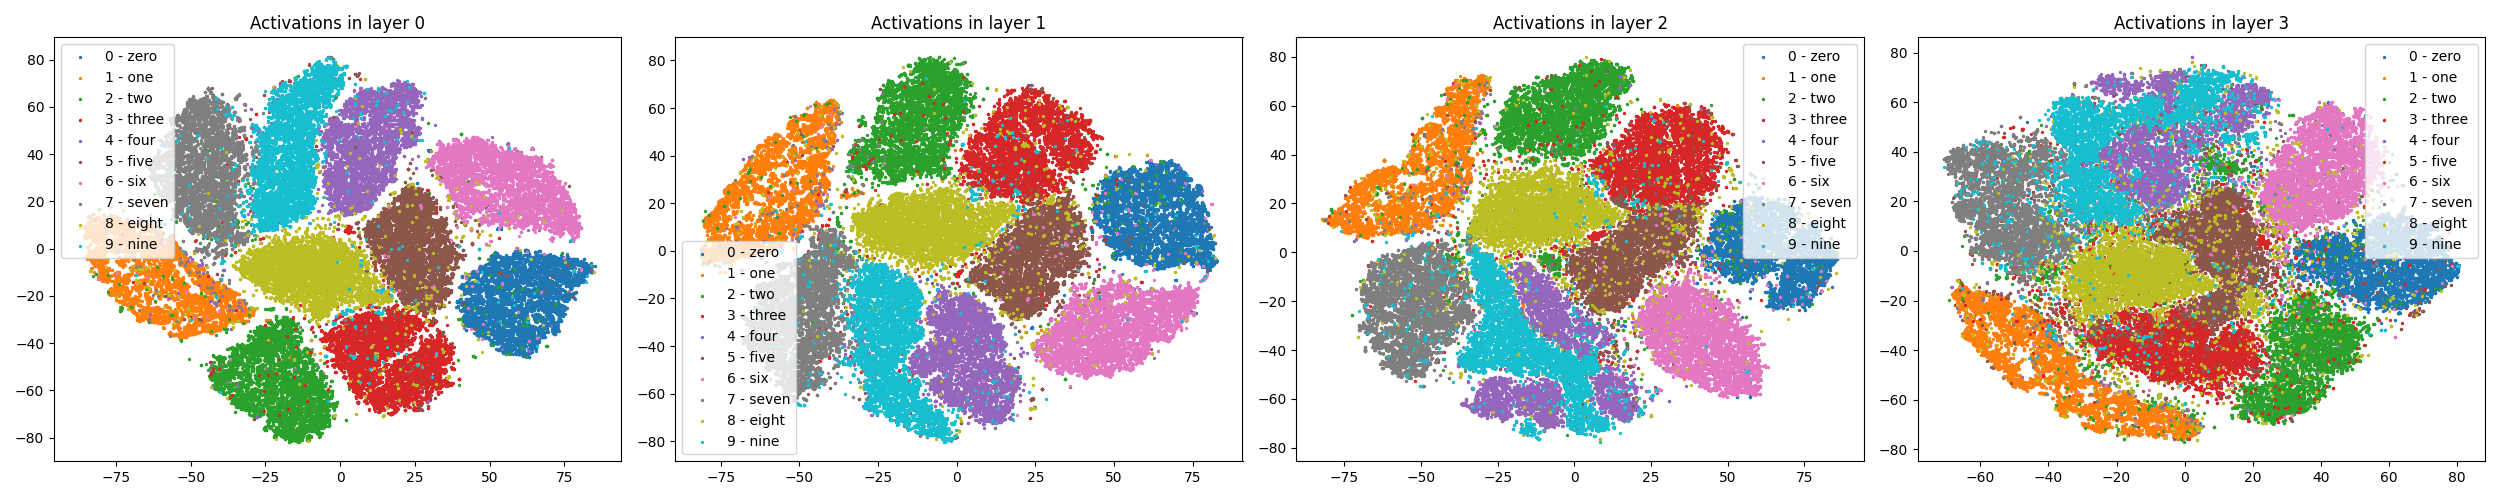
\includegraphics[width=1.0\textwidth]{../../out/activations_feedforward/mnist_t-sne_untrained.png}
  \caption{Embeddings of activations in layers of an untrained neural network (t-SNE).}
\end{figure}

We can observe three trends:
\begin{enumerate}
  \item In the trained network, the representations have a better structure the
      deeper given layer is.
  \item The opposite holds in the untrained network.
  \item The untrained network tends to have worse quality representations.
\end{enumerate}

\begin{figure}
  \centering
    \resizebox{\textwidth}{!}{
        \begin{tabular}{llllll}
\toprule
{} &               ds &               dd &               cs &               cd &          acc\_knn \\
\midrule
layer 0 &  0.3428 / 0.3428 &  1.0732 / 1.0732 &  0.2454 / 0.2454 &  1.0079 / 1.0079 &  0.9713 / 0.9713 \\
layer 1 &  0.3175 / 0.3551 &  1.0761 / 1.0719 &  0.2290 / 0.2531 &  1.0268 / 1.0000 &  0.9861 / 0.9661 \\
layer 2 &  0.3049 / 0.3833 &  1.0775 / 1.0687 &  0.2209 / 0.2731 &  1.0326 / 0.9817 &  0.9915 / 0.9529 \\
layer 3 &  0.3106 / 0.4444 &  1.0768 / 1.0619 &  0.2260 / 0.3159 &  1.0406 / 0.9355 &  0.9911 / 0.9155 \\
\bottomrule
\end{tabular}

    }
  \caption{Values of metrics for embeddings acquired by t-SNE.}
\end{figure}

Aside from computing the embeddings themselves, we also applied the metrics
introduced in the previous section to those embeddings. The table with these
values is shown in Figure 3. There are two values per layer and metric - the
first one corresponds to the trained network, the second one to the untrained
network.

The trends we observed in the plots visually can be seen in the table too. Even
though the effects are not that great, they are consistent.

Next, we will look at embeddings produced by UMAP - these correspond
to Figure 4 and Figure 5.

\begin{figure}
  \centering
    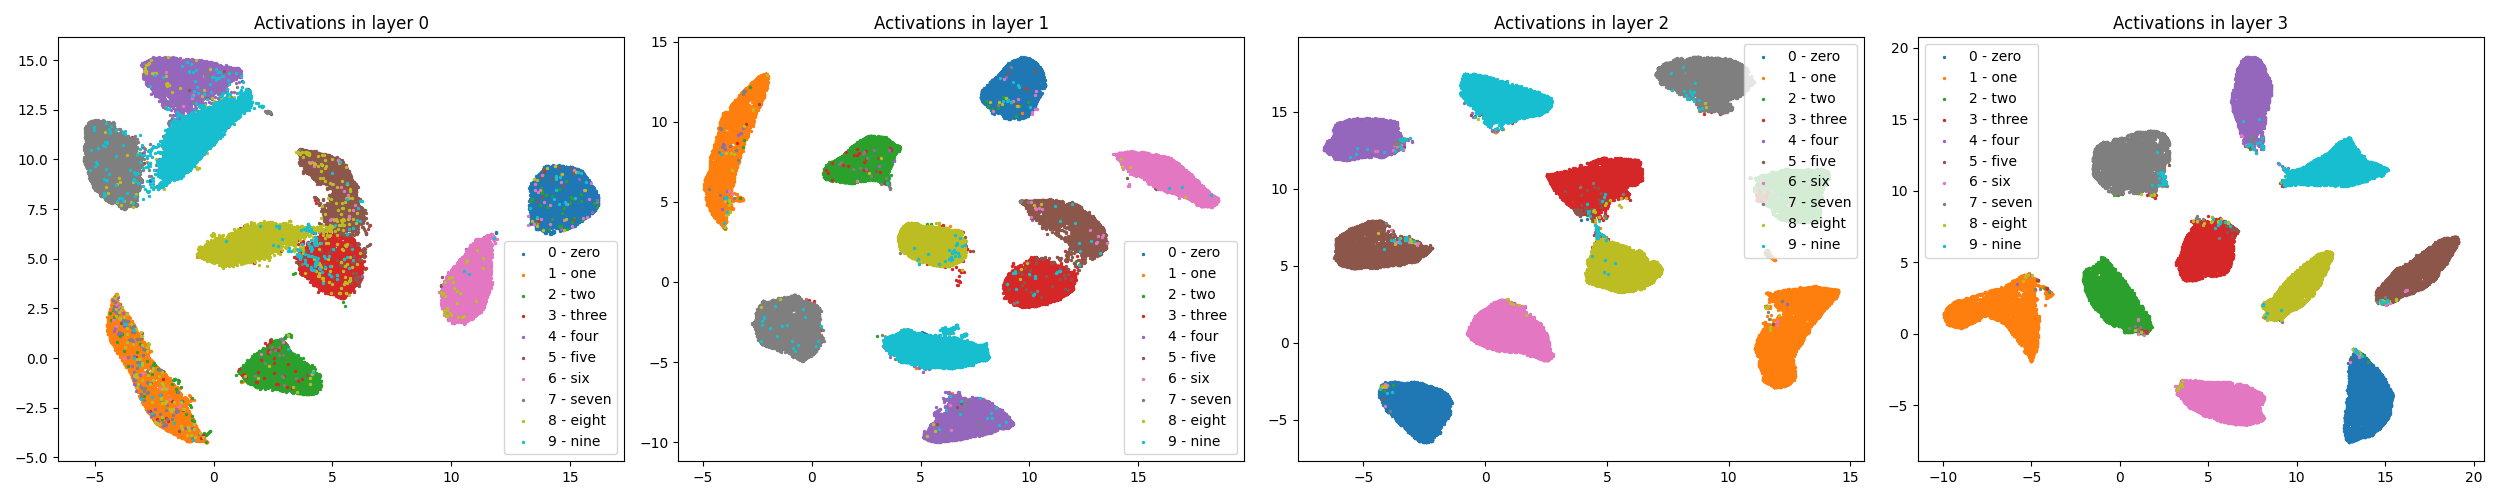
\includegraphics[width=1.0\textwidth]{../../out/activations_feedforward/mnist_umap_trained.png}
  \caption{Embeddings of activations in layers of neural network trained on MNIST (UMAP).}
\end{figure}

\begin{figure}
  \centering
    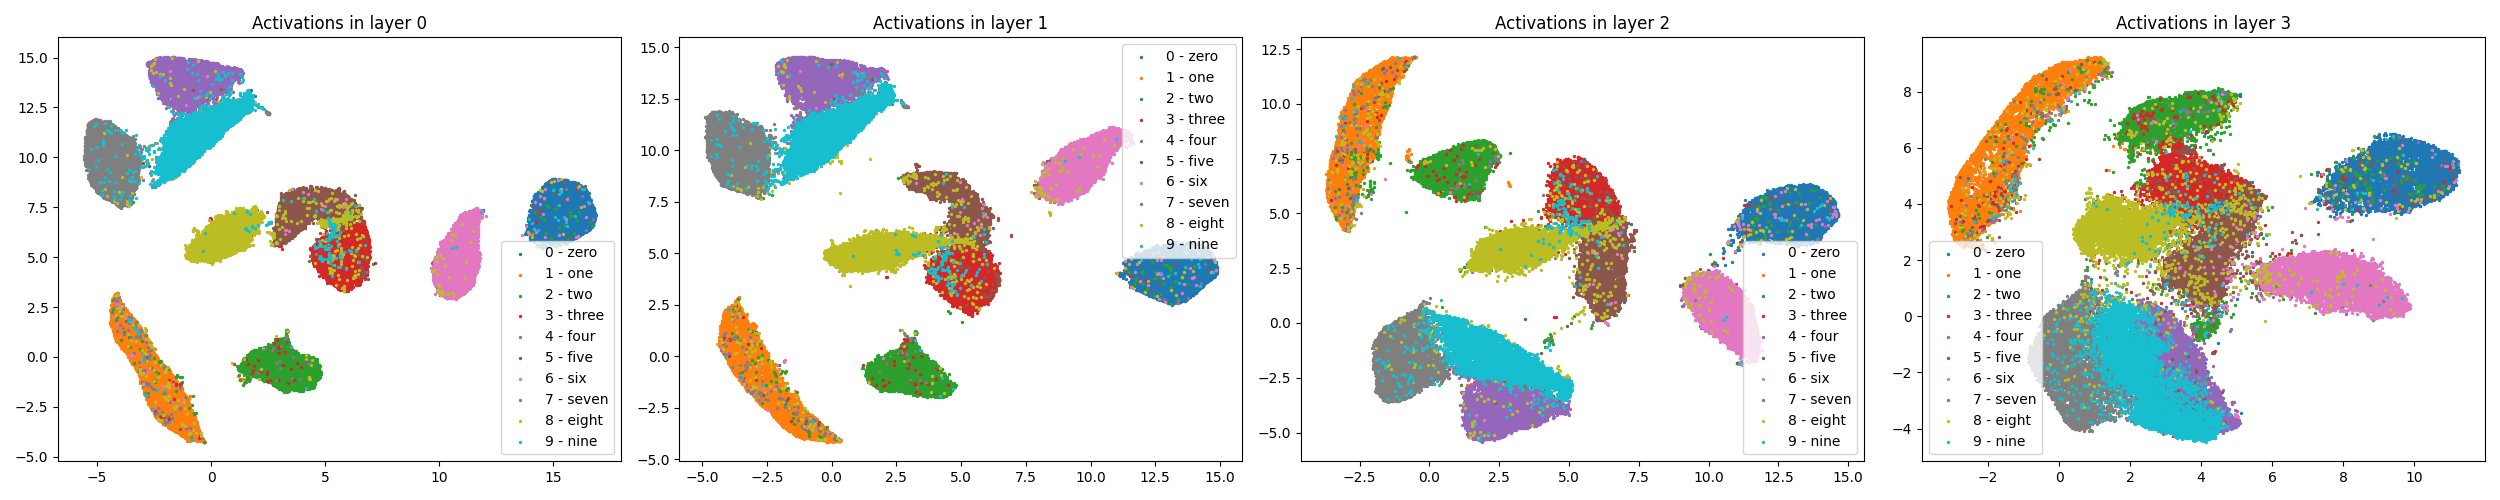
\includegraphics[width=1.0\textwidth]{../../out/activations_feedforward/mnist_umap_untrained.png}
  \caption{Embeddings of activations in layers of untrained neural network (UMAP).}
\end{figure}

The same as in the case of t-SNE can be observed in the case of UMAP. As we get
deeper into the trained network quality of the embeddings gets better, whereas
the deeper we go in the untrained network, the worse is the quality of the
embeddings. We might notice the tendency of UMAP to separate clusters by
a bigger margin; that, however, is of little significance for us.

\begin{figure}
  \centering
    \resizebox{\textwidth}{!}{
        \begin{tabular}{llllll}
\toprule
{} &               ds &               dd &               cs &               cd &          acc\_knn \\
\midrule
layer 0 &  0.2124 / 0.2135 &  1.0878 / 1.0877 &  0.1479 / 0.1486 &  1.0475 / 1.0452 &  0.9688 / 0.9684 \\
layer 1 &  0.1806 / 0.2271 &  1.0913 / 1.0861 &  0.1275 / 0.1577 &  1.0632 / 1.0401 &  0.9852 / 0.9641 \\
layer 2 &  0.1546 / 0.2600 &  1.0942 / 1.0825 &  0.1094 / 0.1801 &  1.0768 / 1.0245 &  0.9911 / 0.9486 \\
layer 3 &  0.1772 / 0.3649 &  1.0917 / 1.0708 &  0.1270 / 0.2568 &  1.0729 / 0.9713 &  0.9908 / 0.8849 \\
\bottomrule
\end{tabular}

    }
  \caption{Values of metrics for embeddings acquired by UMAP.}
\end{figure}

Table with metric values computed from UMAP embeddings can be found in
Figure 6. The effects are very similar to the effects we observed in the case
of t-SNE.

\subsection{FashionMNIST}
Now we are going to do the same except for the FashionMNIST dataset. Again, we
start by observing the embeddings computed using t-SNE - the plots are
shown in Figure 7 and Figure 8.

\begin{figure}
  \centering
    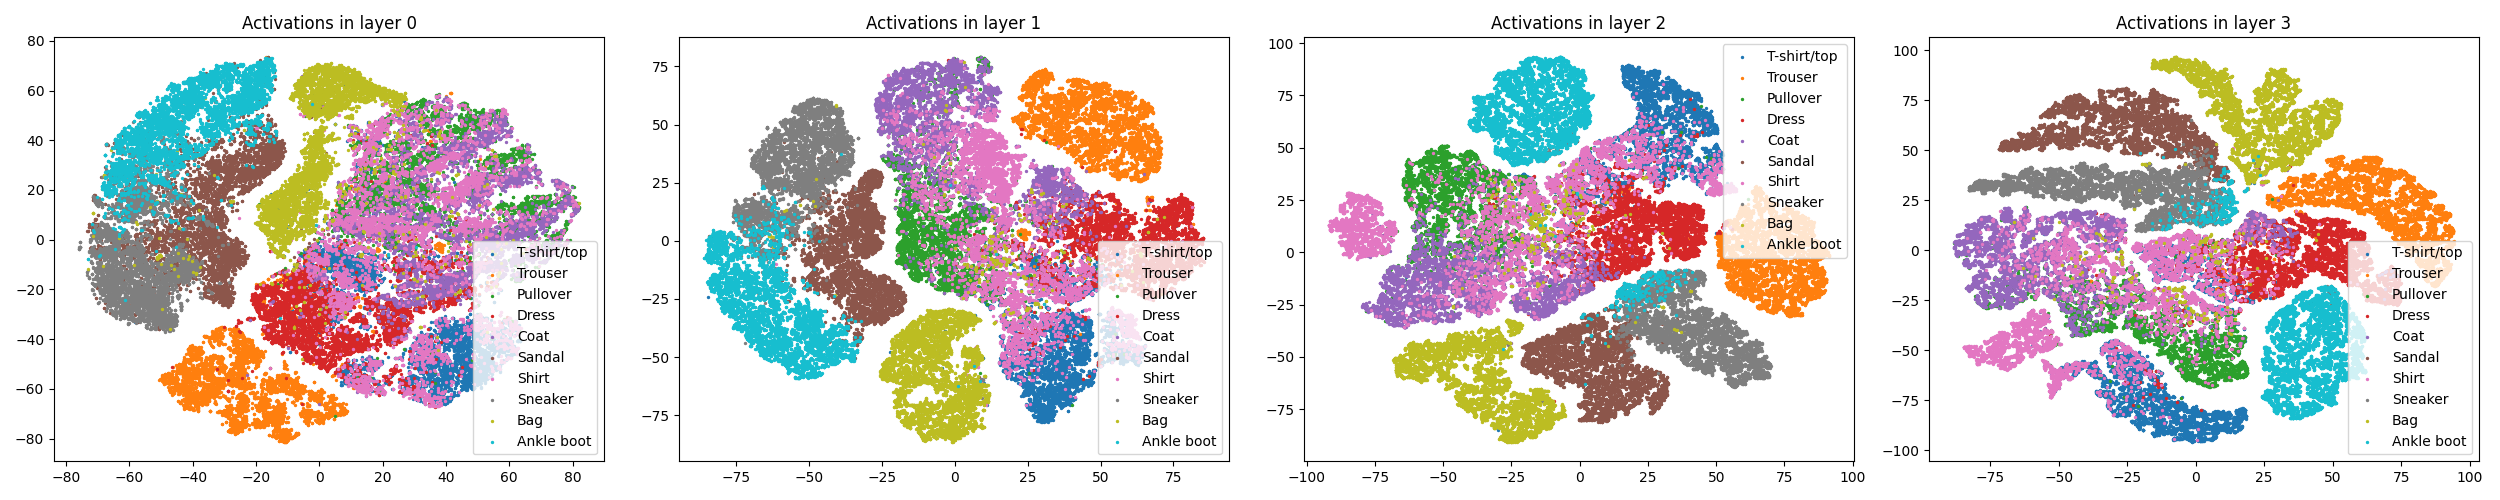
\includegraphics[width=1.0\textwidth]{../../out/activations_feedforward/fmnist_t-sne_trained.png}
    \caption{Embeddings of activations in layers of a neural network trained on FashionMNIST (t-SNE).}
\end{figure}

\begin{figure}
  \centering
    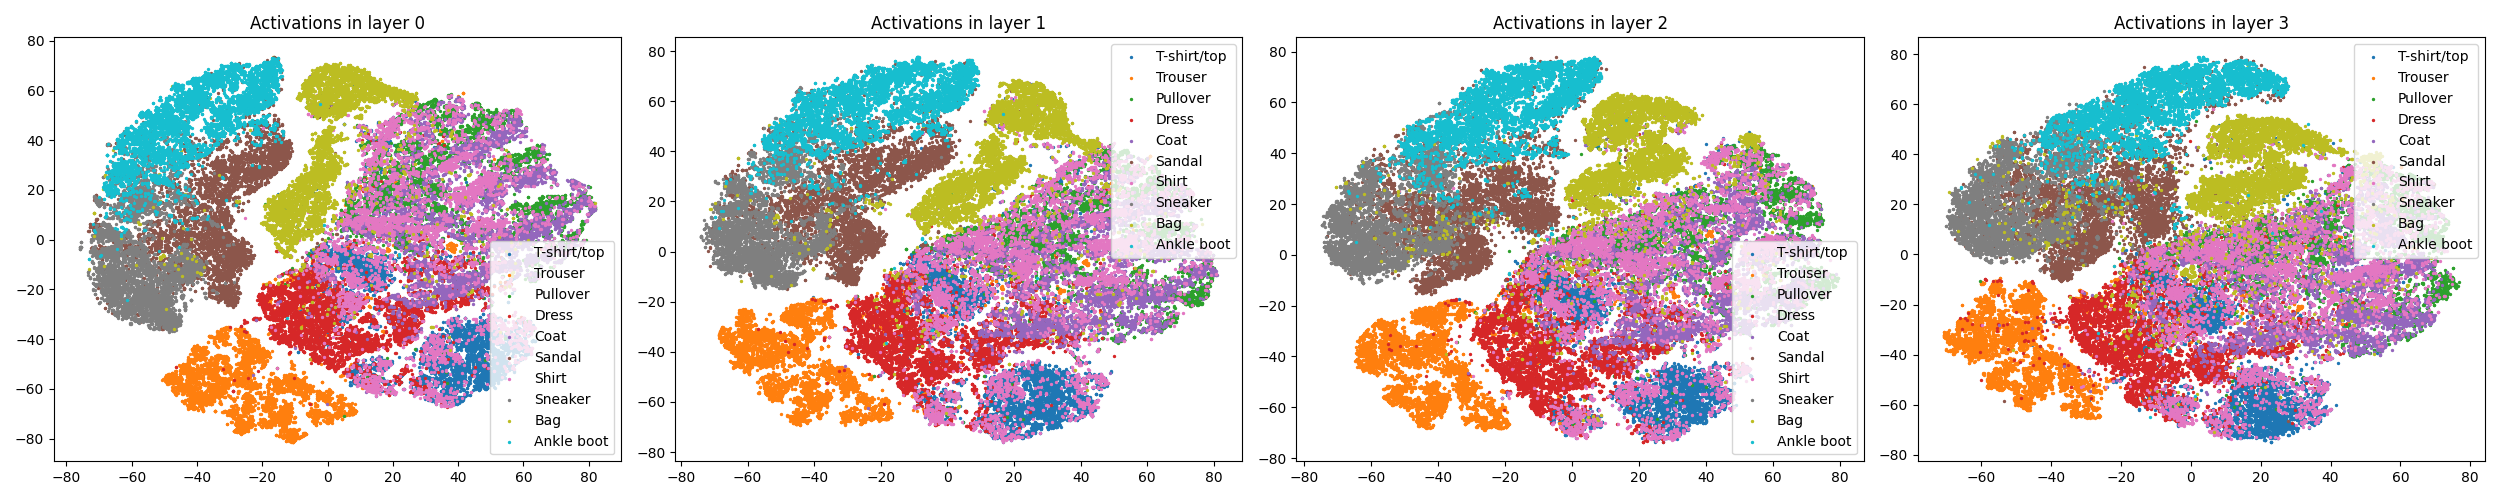
\includegraphics[width=1.0\textwidth]{../../out/activations_feedforward/fmnist_t-sne_untrained.png}
  \caption{Embeddings of activations in layers of an untrained neural network (t-SNE).}
\end{figure}

In this case, the plots are more ambiguous. It is clear that the last
hidden layer of trained network contains activations that have better
structure than the corresponding layer in the untrained network. However, it is
not so clear whether the representations in the last layer are actually
better than the input representations.

\begin{figure}
  \centering
    \resizebox{\textwidth}{!}{
        \begin{tabular}{llllll}
\toprule
{} &               ds &               dd &               cs &               cd &          acc\_knn \\
\midrule
layer 0 &  0.4659 / 0.4659 &  1.0593 / 1.0593 &  0.3439 / 0.3439 &  0.9407 / 0.9407 &  0.8644 / 0.8644 \\
layer 1 &  0.4028 / 0.4648 &  1.0663 / 1.0595 &  0.2950 / 0.3422 &  0.9830 / 0.9419 &  0.8988 / 0.8590 \\
layer 2 &  0.4110 / 0.4645 &  1.0654 / 1.0595 &  0.2980 / 0.3396 &  0.9725 / 0.9412 &  0.8976 / 0.8484 \\
layer 3 &  0.4432 / 0.4755 &  1.0619 / 1.0583 &  0.3245 / 0.3462 &  0.9568 / 0.9349 &  0.8955 / 0.8324 \\
\bottomrule
\end{tabular}

    }
  \caption{Values of metrics for embeddings acquired by t-SNE.}
\end{figure}

To get a better picture, we take a look at the table in Figure 9. Once again,
we see that the quality of representations follows the same trend as before.
However, this time the effects are noticeably less profound.

Again, we will also look at the embeddings computed by UMAP. These can be seen
in Figures 10 and 11.

\begin{figure}
  \centering
    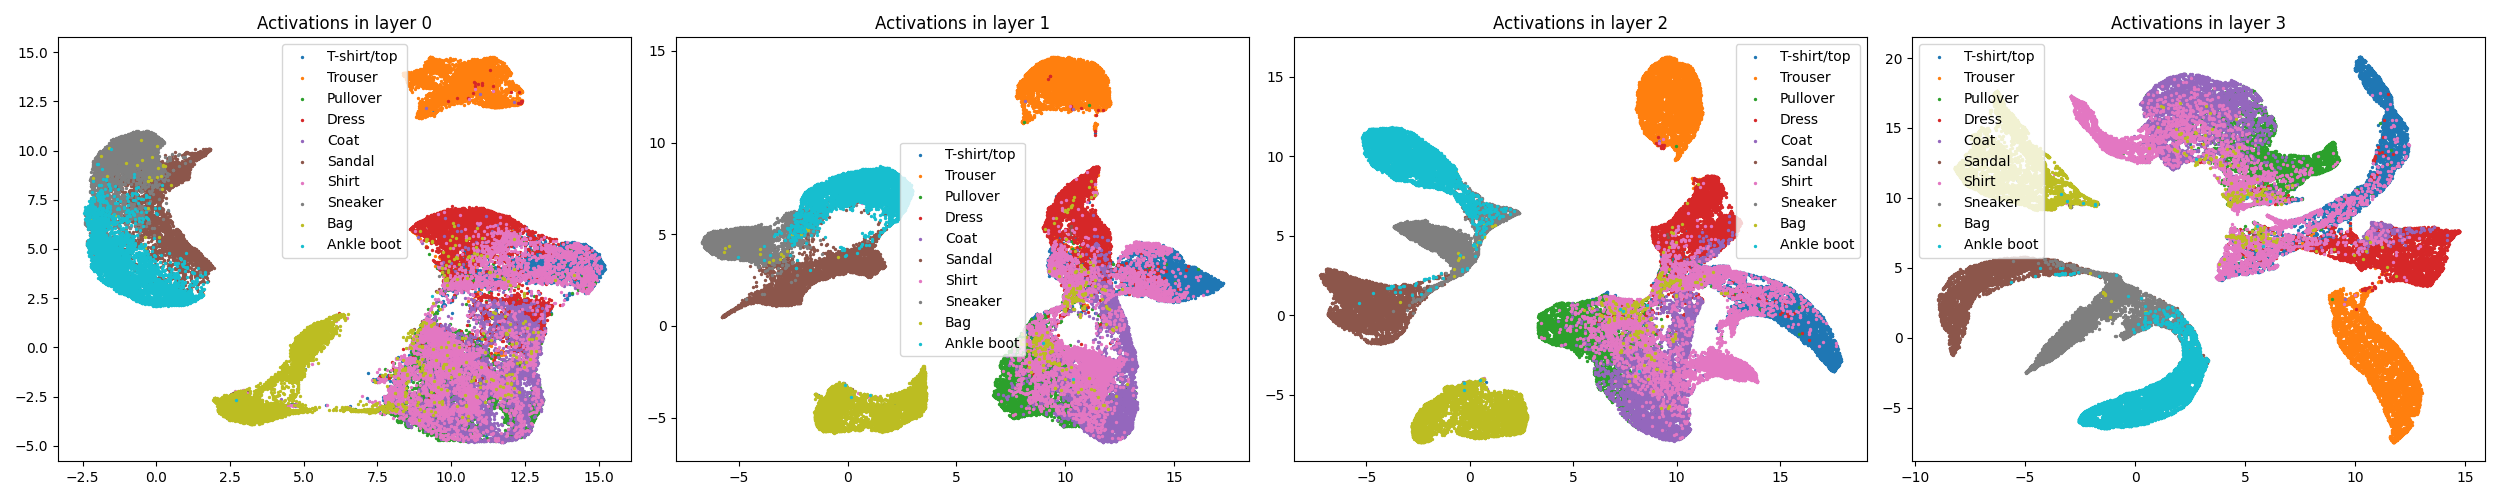
\includegraphics[width=1.0\textwidth]{../../out/activations_feedforward/fmnist_umap_trained.png}
  \caption{Embeddings of activations in layers of neural network trained on FashionMNIST (UMAP).}
\end{figure}

\begin{figure}
  \centering
    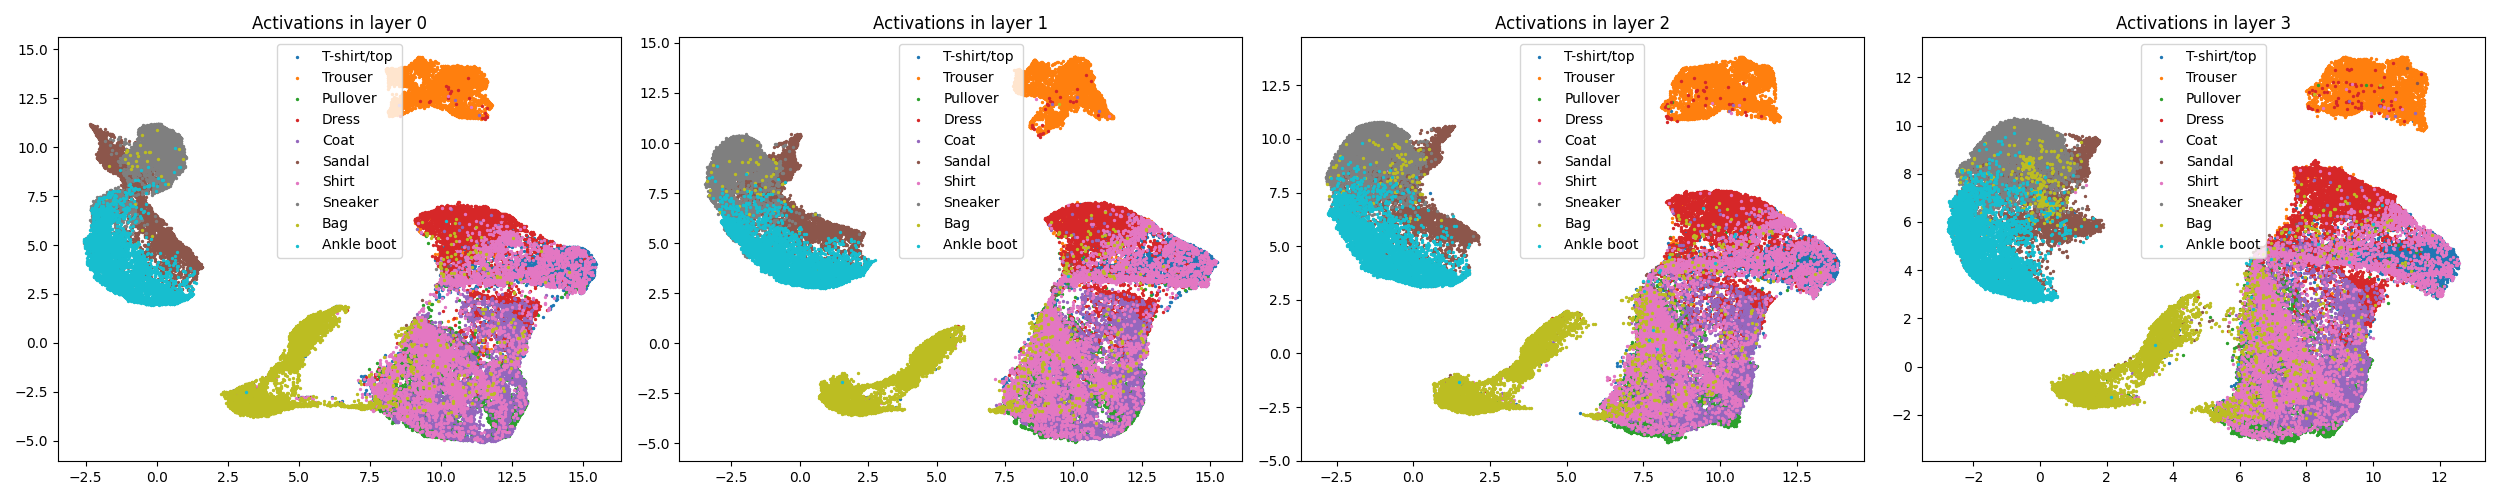
\includegraphics[width=1.0\textwidth]{../../out/activations_feedforward/fmnist_umap_untrained.png}
  \caption{Embeddings of activations in layers of untrained neural network (UMAP).}
\end{figure}

In this case, the plots do not give us a definite answer concerning the
quality of representations extracted from neural networks. It is very hard
to tell from the plots alone whether the quality of representations improved
or not.

\begin{figure}
  \centering
    \resizebox{\textwidth}{!}{
        \begin{tabular}{llllll}
\toprule
{} &               ds &               dd &               cs &               cd &          acc\_knn \\
\midrule
layer 0 &  0.2994 / 0.3046 &  1.0778 / 1.0773 &  0.2208 / 0.2254 &  1.0197 / 1.0165 &  0.8122 / 0.8130 \\
layer 1 &  0.2602 / 0.3030 &  1.0822 / 1.0774 &  0.1895 / 0.2224 &  1.0433 / 1.0182 &  0.8836 / 0.8075 \\
layer 2 &  0.2693 / 0.3230 &  1.0812 / 1.0752 &  0.1942 / 0.2362 &  1.0421 / 1.0086 &  0.8912 / 0.7901 \\
layer 3 &  0.3328 / 0.3470 &  1.0741 / 1.0725 &  0.2444 / 0.2521 &  1.0084 / 0.9963 &  0.8924 / 0.7729 \\
\bottomrule
\end{tabular}

    }
  \caption{Values of metrics for embeddings acquired by UMAP.}
\end{figure}

The table with metric values is shown in Figure 12. Again, we see
a consistent trend regarding the quality of embeddings. The effects are not
significant in most cases. However, in the case of the accuracy of the k-nearest
neighbor classifier, we see a noticeable difference in performance when
using different representations.

\section{Conclusions}
In this work, we attempted to tackle the problem of data representation using
activations of a neural network. To find out whether these representations
are superior to their original counterparts, we compared them both visually
and using several metrics of embedding quality.

We found out that although there is a consistent trend of increasing the quality
of representations when increasing the depth at which the activations were
acquired from the neural network, the effects are rather small.

\section{Future work}
This work only used a single neural network architecture. Moreover, the
architecture is not even suitable for the task at hand; the use of
a convolutional neural network would make more sense with respect to the
problem structure. It would also be interesting to see whether the
representations of such networks would provide different results. Thus use
of different architecture, coupled with varying its hyperparameters like
loss function and layer width, would seem like a reasonable step forward.

The metrics used in this work are rather arbitrary and not based on a formal
framework. This makes their ability to assess the quality of embeddings
questionable at best. Better metrics and an overall more comprehensive analysis
of the representations could help us better understand in what way are the new
representations different and in what ways they could be used.

\end{document}



















